
\section{Dataset}
This section introduces how we build the whole dataset from raw data.

TODO: 这里插一张总体流程图

\subsection{Data Description}
Our data is taken from the records of GPS devices on the taxis in Shenzhen. A brief description is as the following:
\begin{itemize}
    \item \textbf{Region:} Shenzhen
    \item \textbf{Time Range:} June 2020
    \item \textbf{Content:} Taxi GPS records
    \begin{itemize}
      \item License number
      \item Longitude and latitude
      \item Speed
      \item Timestamp
      \item $\cdots$
    \end{itemize}
  \item \textbf{Size:} Over 2,500,000,000 rows
\end{itemize}

A small part of data is shown as an example in figure \ref{fig: raw_data}.
\begin{figure}[htb]
    \centering
    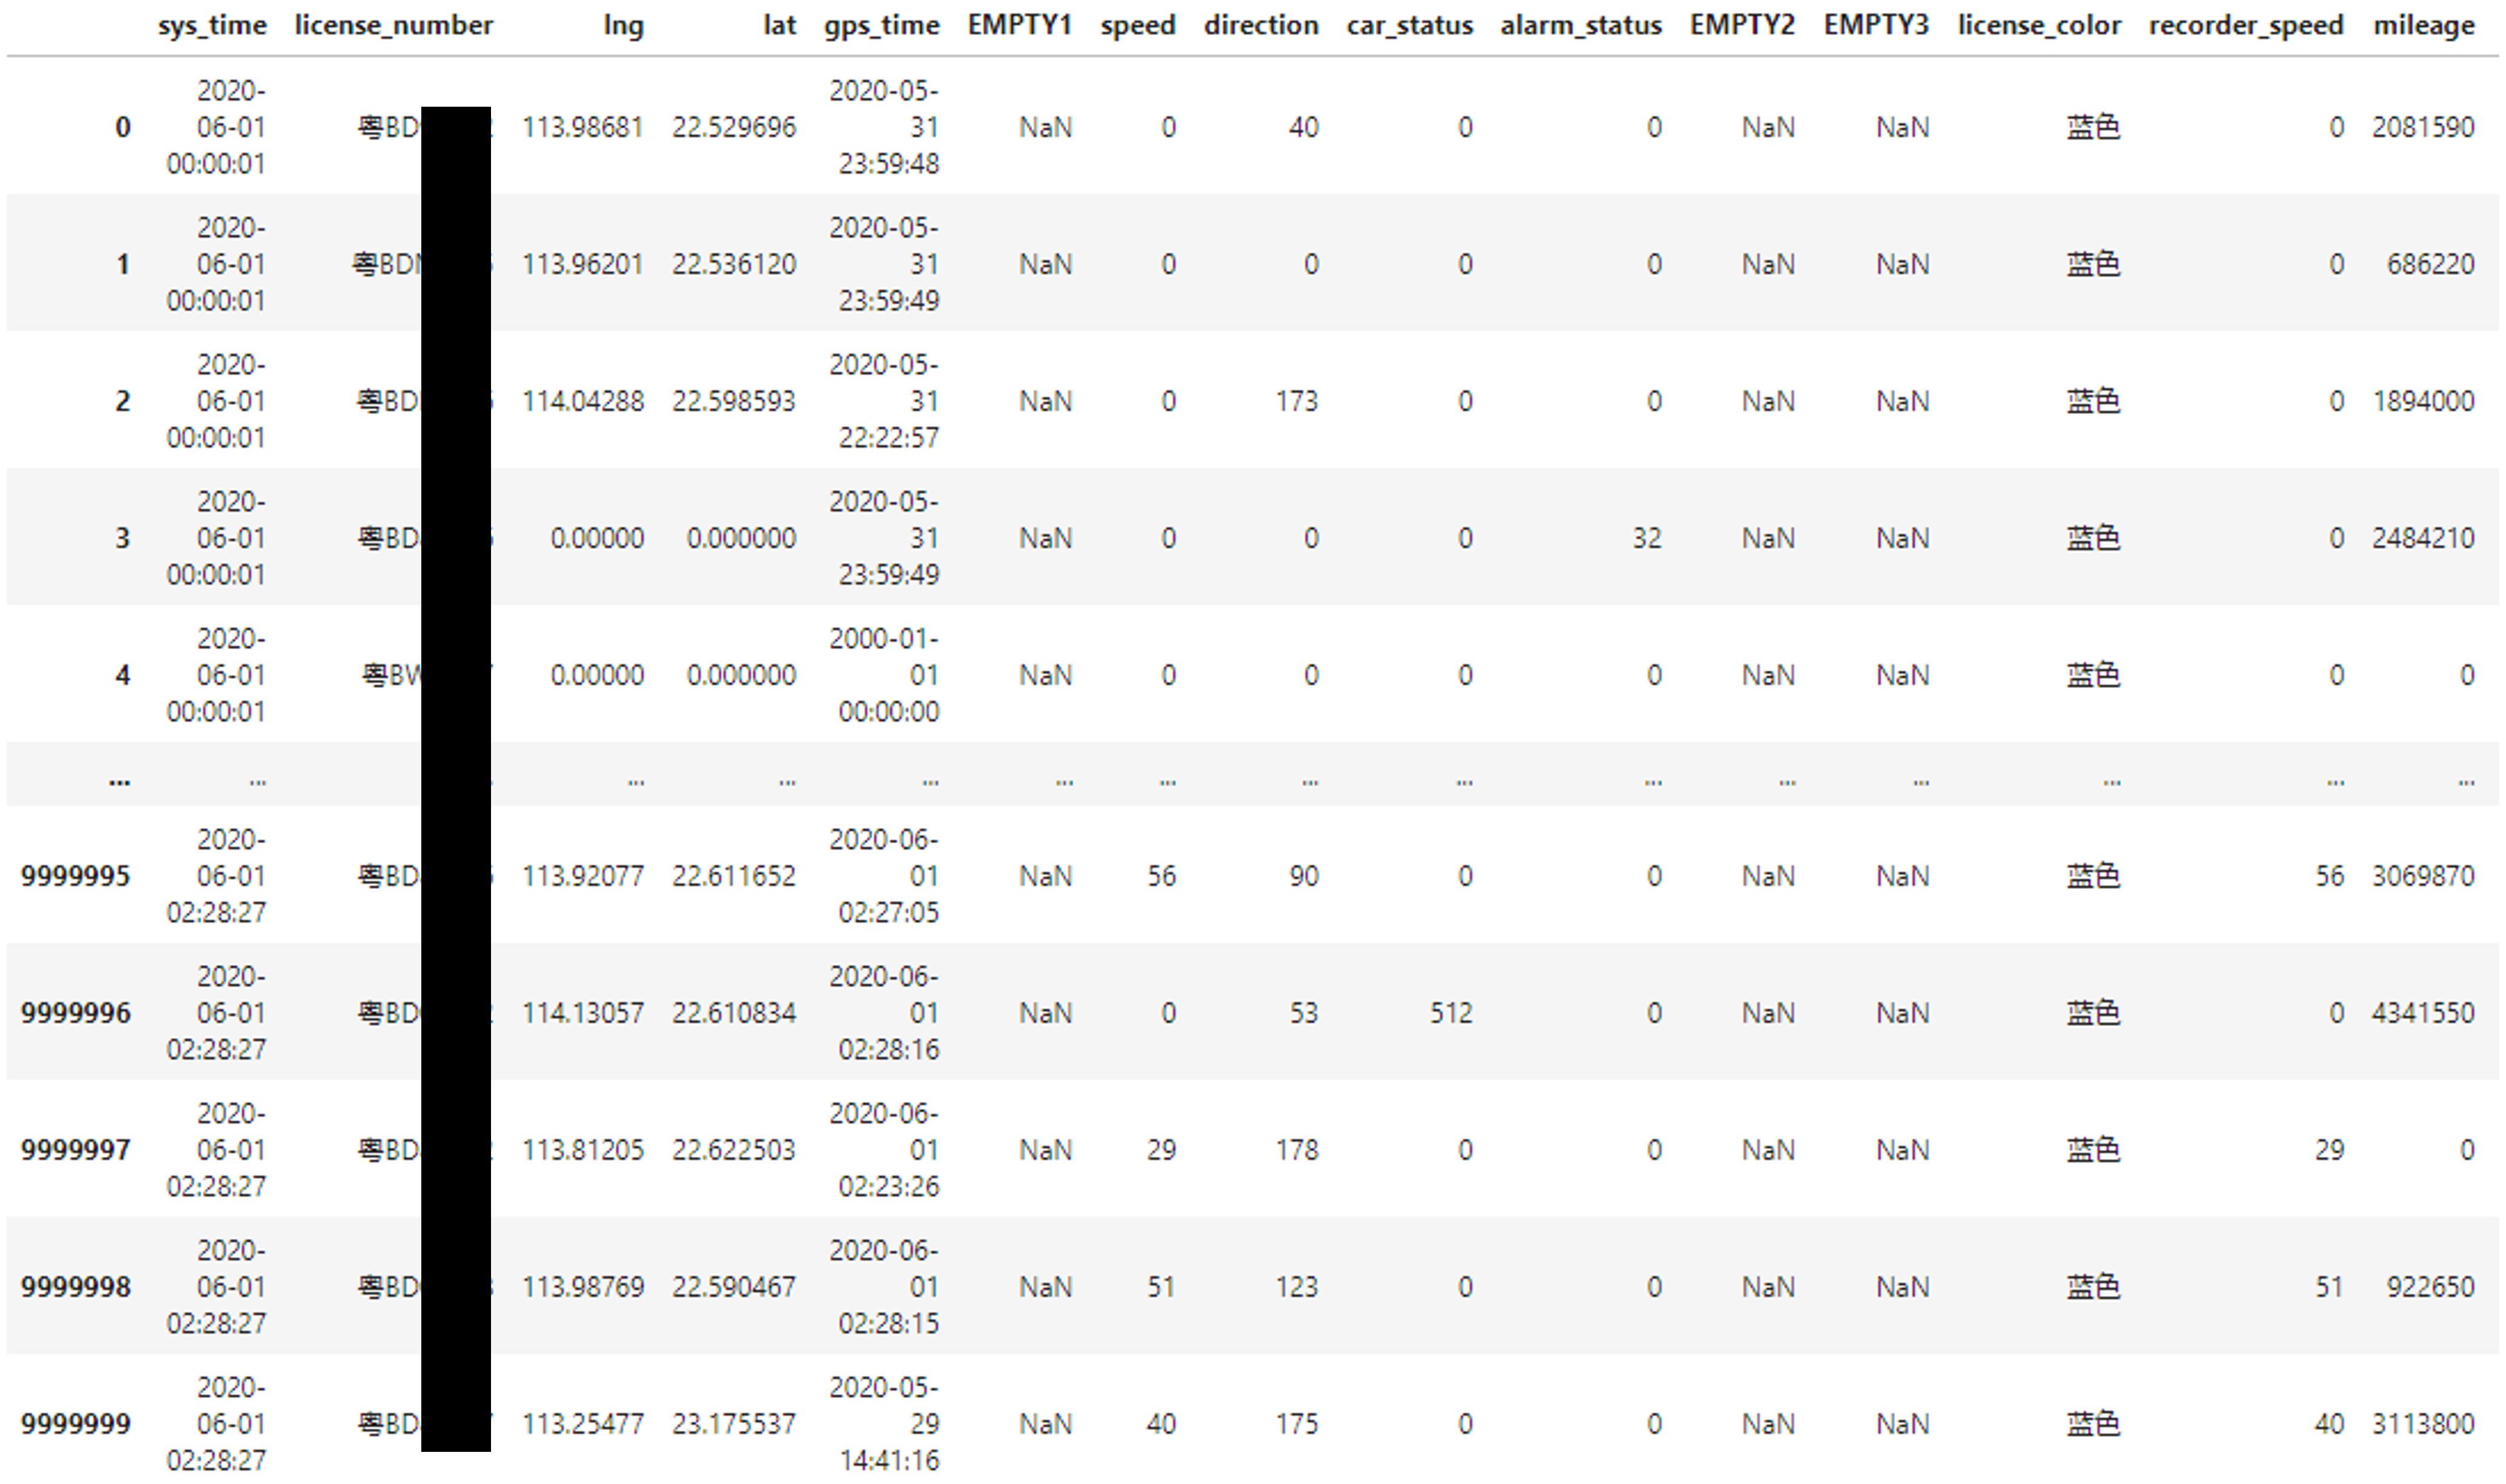
\includegraphics[width=\textwidth]{images/raw_data.png}
    \caption{Shenzhen taxi GPS raw data}
    \label{fig: raw_data}
\end{figure}

Unlike the open datasets that can be applied to deep learning models without the need of data cleaning and completion, this raw dataset contains lots of abnormal values, which should be cleaned and re-organized carefully.

\subsection{Data Cleaning}
Data cleaning is the process of detecting and correcting (or removing) corrupt or inaccurate records from a record set, table, or database and refers to identifying incomplete, incorrect, inaccurate or irrelevant parts of the data and then replacing, modifying, or deleting the dirty or coarse data\cite{data_cleaning}. There are many kinds of bad records that should be deleted or modified. To summarize, we categorize them as the following classes.

\begin{enumerate}
  \item \textbf{Duplicate Rows.} A considerable large part of the raw data are duplicate. The reason is when a GPS device is transmitting data to server, it will send several copies in order to avoid packet loss under poor Internet connection. As a result, they are completely same rows, and thus can be removed safely, leaving only the foremost one.
  \item \textbf{Corrupted Timestamp.} This is a sort of abnormal record. Since our time range is June 2020, all the timestamps that not in here should be deleted. In detail, there are two kinds of them: 1) records in May $31^{st}$ or July $1^{st}$. This is caused by the equipments' lack of accuracy. 2) 2000-01-01. And this is caused by data loss, thus, it is filled by a default value.
  \item \textbf{Missing Location.} The latitude and longitude of some records are zero, which is resulted by the data loss during transmission. These dirty values should be deleted.
  \item \textbf{Zero Speed.} Stationary taxis are still transmitting their location information to the server if the GPS device is on, leading to a big portion of zero speed records. They are useless owing to that trajectories are a series of moving locations. Therefore, under normal circumstances, it is better to remove them. However, things are not that happy in our data. There are four kinds of zero speed records relating to the change of location, i.e. latitude and longitude, and they should be treated differently. Details are provided in the next subsection.
  \item \textbf{Irrelevant Attributes.} As shown in figure \ref{fig: raw_data} above, the raw data consists of several columns. The information that have no contribution to trajectories needs to be removed, leaving only latitude, longitude, speed and timestamp.
\end{enumerate}

We take the data of June $1^{st}$ as a case study to give an illustration of our data cleaning procedure and hope to reflect the property of the whole GPS data. In total, there are 97,453,725 rows. Table \ref{data_cleaning_table} gives the deleted percentage and remaining rows after each data cleaning step.

\begin{table}[htb]
  \begin{center}
      \caption{Data Cleaning Example on June $1^{st}$}
      \label{data_cleaning_table}
      \begin{tabular}{ccc}
          \toprule

          \textbf{Step} & \textbf{Deleted Percentage} & \textbf{\#Remaining Rows}\\

          \midrule

          Drop duplicate & $51.73\%$ & 47,042,104\\
          Drop abnormal values & $1.19\%$ & 45,874,548\\
          Drop zero speed & $16.84\%$ & 29,458,603\\

          \cmidrule{1-2}

          \textbf{Remaining Percentage} & $30.22\%$ & ~\\

          \bottomrule
      \end{tabular}
  \end{center}
\end{table}

As shown in the table, half of the records are duplicated. Fortunately the total number of records are large enough to endure the data cleaning procedure. For the $17\%$ zero speed records, the following figure points out the huge impact of removal on the distribution of speed.

\subsection{Data Processing}
